\documentclass[14pt,oneside]{extarticle}
\usepackage[utf8]{inputenc}
\usepackage[english,russian]{babel}
\usepackage[backend=biber,style=numeric]{biblatex}
\addbibresource{src/bibliography.bib}
\usepackage{geometry}
\geometry{
    a4paper,
    total={170mm,257mm},
    left=30mm,
    top=20mm,
    right=15mm,
    bottom=20mm,
}

\usepackage{fancyhdr}
\pagestyle{fancy}
\renewcommand\headrulewidth{0pt} % no line between document and header
\fancyhead{} % clear header
\fancyfoot{} % clear footer
\fancyfoot[LE,RO]{\thepage}

\usepackage{listings}
\lstset{
    basicstyle=\footnotesize\ttfamily,
    frame=single,
    tabsize=4,
}
\newcommand{\inlinecode}{\lstinline[basicstyle=\normalsize\ttfamily]}

\usepackage{graphicx}

\usepackage{indentfirst}
\parindent=1cm

\renewcommand{\labelenumii}{\theenumii}
\renewcommand{\theenumii}{\theenumi.\arabic{enumii}.}

\begin{document}
    \begin{titlepage}
    \begin{center}
        МИНИСТЕРСТВО И НАУКИ И ВЫСШЕГО ОБРАЗОВАНИЯ РОССИЙСКОЙ ФЕДЕРАЦИИ\\
        Федеральное государственное автономное образовательное\\
        учреждение высшего образования

        \textbf{
        <<Южно-Уральский Государственный университет\\
        (национальный исследовательский университет)>>\\
        Высшая школа электроники и компьютерных наук\\
        Кафедра системного программирования
        }
        \bigskip
        
        \noindent
        \newline
        \begin{minipage}{0.5\textwidth}
            РАБОТА ПРОВЕРЕНА\\
            Рецензент,\\
            Программист ООО "Бонапарт"\\
            \underline{\hspace{2cm}} М.А. Тармин\\
            «\underline{\hspace{0.7cm}}» \underline{\hspace{2cm}} 2020 г.
        \end{minipage}
        \vspace{\fill}
        \begin{minipage}{0.4\textwidth}
            ДОПУСТИТЬ К ЗАЩИТЕ\\
            Заведующий кафедрой,\\
            д.ф.-м.н., профессор\\
            \underline{\hspace{2cm}} Л.Б. Соколинский\\
            «\underline{\hspace{0.7cm}}» \underline{\hspace{2cm}} 2020 г.
        \end{minipage}

        \vfill
        \large\textbf{
            РЕИНЖИНИРИНГ КОНСУЛЬТАЦИОННОГО ЧАТ-БОТА ДЛЯ КЛИЕНТОВ ТОРГОВОЙ КОМПАНИИ
        }        
        \bigskip
        
        ВЫПУСКНАЯ КВАЛИФИКАЦИОННАЯ РАБОТА\\
        ЮУрГУ – 02.04.02.2020.308-149.В
    \end{center}
    \vfill

    \hfill
    \begin{minipage}{0.4\textwidth}
        Научный руководитель\\
        \underline{\hspace{2cm}} Н.Ю. Долганина\\
        «\underline{\hspace{0.7cm}}» \underline{\hspace{2cm}} 2020 г.
    \end{minipage}
    \bigskip
    \vfill

    \hfill
    \begin{minipage}{0.4\textwidth}
        Автор работы,\\
        студент группы КЭ-220\\
        \underline{\hspace{2cm}} Н.В. Плющай\\
        «\underline{\hspace{0.7cm}}» \underline{\hspace{2cm}} 2020 г.
    \end{minipage}
    \bigskip
    \vfill

    \hfill
    \begin{minipage}{0.4\textwidth}
        Ученый секретарь\\
        (нормоконтролер)\\
        \underline{\hspace{2cm}} О.Н. Иванова\\
        «\underline{\hspace{0.7cm}}» \underline{\hspace{2cm}} 2020 г.
    \end{minipage}
    \bigskip
    \vfill

    \begin{center}
        Челябинск, 2020
    \end{center}
\end{titlepage}

    \begin{titlepage}
    
    \begin{center}
        \footnotesize
        МИНИСТЕРСТВО НАУКИ И ВЫСШЕГО ОБРАЗОВАНИЯ РОССИЙСКОЙ ФЕДЕРАЦИИ\\
        \small
        Федеральное государственное автономное образовательное\\
        учреждение высшего образования\\
        \normalsize
        \textbf{
        <<Южно-Уральский Государственный университет\\
        (национальный исследовательский университет)>>\\
        \small
        Высшая школа электроники и компьютерных наук\\
        Кафедра системного программирования
        \normalsize
        }
        \bigskip
    \end{center}

    \hfill
    \begin{minipage}{0.4\textwidth}
        УТВЕРЖДАЮ\\
        Заведующий кафедрой,\\
        \underline{\hspace{2cm}} Л.Б. Соколинский\\
        09.02.2020
    \end{minipage}

    \begin{center}
        \textbf{ЗАДАНИЕ}\\
        \textbf{на выполнение выпускной квалификационной работы магистра}\\
        студенту группы КЭ-220\\
        Плющай Николаю Владимировичу,\\
        обучающемуся по направлению\\
        02.04.02 «Фундаментальная информатика и информационные технологии»\\
        (магистерская программа «Технологии разработки высоконагруженных систем»)\\
    \end{center}

    \begin{enumerate}
        \item \textbf{Тема работы:} (Утверждена приказом ректора от 24.04.2020 №627)\\
        Реинжиниринг консультационного чат-бота для клиентов торговой компании.
        \item \textbf{Срок сдачи студентом законченной работы:} 5.06.2020.
        \item \textbf{Исходные данные к работе:}
        \begin{enumerate}
            \item М. Фаулер Улучшение существующего кода // Символ-Плюс, 2003.
            \item С. Макконнел Совершенный код // Microsoft Press, 2017.
            \item Э. Гамма и др. Приемы объектно-ориентированного проектирования // Питер, 2015.
        \end{enumerate}
        \item \textbf{Перечень подлежащих разработке вопросов}
        \begin{enumerate}
            \item Произвести анализ исходного проекта.
            \item Выявить проблемные места.
            \item Составить план проведения работ.
            \item Изучить современные подходы и средства разработки.
            \item Спроектировать систему чат-бота.
            \item Реализовать, протестировать и развернуть новую систему.
            \item Провести анализ выполненной работы.
        \end{enumerate}
        \item \textbf{Дата выдачи задания:} 24.04.2020.
    \end{enumerate}

    \noindent\\
    \textbf{Научный руководитель}\\
    Доцент кафедры СП, к.т.н. \hfill Н.Ю. Долганина
    
    \noindent\\
    \textbf{Задание принял к исполнению} \hfill Н.В. Плющай

    \thispagestyle{empty}
\end{titlepage}
    \tableofcontents
    
    % введение
    \addcontentsline{toc}{section}{ВВЕДЕНИЕ}
\section*{ВВЕДЕНИЕ}
Обработка естественных языков (\textit{Natural Language Processing, NLP})
-- направление компьютерной лигвистики и машинного обучния,
изучающее анализ и синтез естественных языков.
Под обработкой естественных языков  понимается создание систем,
обрабатывающих естественные языки с целью выполнения определенных задач.
В список этих задач могут входить \cite{cursera.nlp}:
\begin{itemize}
    \item Формирование ответов на вопросы (\textit{Question Answering})
    \item Анализ эмоциональной окраски высказываний (\textit{Sentiment Analysis})
    \item Машинный перевод (\textit{Machine Translation})
    \item Распознавание речи (\textit{Speech Recognition})
    \item Морфологическая разметка (\textit{Part of Speech Tagging})
    \item Извлечение сущностей (\textit{Name Entity Recognition})
\end{itemize}

Диалоговые системы -- это системы, решающие задачу формирвания отвеов на вопросы.
Само формирование ответов может споровождаться решением сопутствующих задач, таких как
извлечение именнованных сущностей или анализ эмоциональной окраски.
Диалоговые системы можно охарактеризовать по двум векторам:
задача-ориентированная или общего назначения (\textit{task-oriented/general})
и закрытого или открытого диапазона тем (\textit{closed/open domain}).
Первая классификация определяет создани ли система для решения одного конкретного
вопроса по данной теме в ходе диалога, или позваляет свободно вести продолжительный
диалог на поставленную тему.
Вторая классификация определяет на сколько диалоговая система ограничена в диапазоне выбора тем
для беседы с человеком.

Чат-боты -- это диалоговые системы, обладающие интерфесом для взаимодействия с человеком.
Чаще всего чат-боты работают через мессенджеры, социальные сети, форумы или диалоговые окна на сайтах.
Также, чаще всего боты используются для решения типовых задач, хорошо описываемых сценариями.
Такие чат-боты часто применяются в бизнесе для оперативного решения вопросов клиентов.
Чат-боты со свободной темой диалога чаще используются для развлечения.

Клиентские чат-боты предназначены для взаимодействия с клинтами той или иной организации,
оперативного и массового решения вопросов клиента, либо сбора информации
для оформления лучшего предолжения.

Чат-бот, рассматриваемый в этой работе, относится к клиентским чат-ботам,
имеет четкий список тем для диалогов и шаблоны ответов, что позволяет отнести
его к группе, так называемых, авто-информаторов.

    % анализ предметной области
    \section{АНАЛИЗ ПРЕДМЕТНОЙ ОБЛАСТИ}
    \subsection{Анализ исходных данных}
    Существующий проект выполняет задачи сбора сообщений с социальных сетей, мессенджеров и почты,
    их классификации и рассылки ответов пользователям.
    Проект оснащен системой непрерывной сборки и развертывания (CI/CD Pipeline), интегрированной в
    систему управления репозиториями \textit{GitLab}.
    Кодовая база проекта, как и сам проект, разделены на пять репозиториев с различными
    функциональными частями.
    
    Ниже представлен их список:
    \begin{enumerate}
        \item Приложения по работе с каналами
        \item API чат-бота для внешнего использования
        \item Диалоговая система чат-бота
        \item Система мониторинга и разметки сообщений
        \item Прокси-сервер и мониторинг нагрузки
    \end{enumerate}
    
    Все приложения собираются и разворачиваются внутри docker-контей-неров.
    Приложения по работе с каналами выполнены на языке \textit{Python} как асинхронные приложения
    с использованием библиотеки \textit{asyncio} и асинхронных библиотек.
    API чат-бота выполнено также на языке \textit{Python} с использованием веб-фреймворка \textit{Flask}.
    Оба эти подпроекта используют диалоговую систему, в которой реализован непосредственный
    классификатор сообщений.
    Диалоговая система импортируется как библиотечный модуль через внутренний репозиторий
    программного обеспечения \textit{PyPI}.
    При появлении обновления в репозитории диалоговой системы срабатывает триггер CI/CD пайплайна
    в приложениях каналов и API, и их конейнеры пересобираются с новой версией библиотеки.
    Система мониторинга реализована на языке \textit{Python} как \textit{Django} веб-приложение.
    Для мониторинга используется администраторская доска управления \textit{Django} приложения.
    В ней же реализован подсчет статистики и \textit{SQL-explorer} для запросов в базу данных.
    Прокси-сервер работает поверх всех сервисов, а именно: API-сервис, система мониторинга,
    системы оповещения и мониторинга ошибок \textit{Sentry}, система мониторинга нагрузки \textit{Prometheus}
    с выводом графики через \textit{Grafana}. Он перераспределяет http-запросы к поддоментам на конкретные
    приложения и сервисы.

    Функциональная схема проекта представлена на рисунке ниже.
    \begin{figure}[!h]
        \centering
        % \includegraphics[width=\linewidth]{}
        \caption{Функциональная схема исходного проекта}
        \label{fig:func-schema-before}
    \end{figure}
    
    Разберем подробнее основные функциональные элементы, это: приложение по работе с каналами, API-сервис и диалоговую систему.
    
    \subsubsection{приложение по работе с каналами}
    Приложение работает по трем каналам: Вконтакте, Телеграм и почта. Логику работы всех трех каналов можно обощить
    следующим образом: в цикле поочередно обрабатываются входящие  и исходящие письма, входящие письма дополнительно
    классифицируются, к ним вырабатывается и отправляется ответное сообщение, затем входящее или исходящее сообщение
    сохраняется в базу. Для сохранения в базу используется библиотека \textit{}, сохранение происходит через формирование
    сырого SQL-запроса.
    
    Для канала Вконтакте используется библиотека \textit{}, функциональная схема представлена ниже:
    \begin{figure}[!h]
        \centering
        % \includegraphics[width=\linewidth]{}
        \caption{Функциональная схема канала Вконтакте}
        \label{fig:func-schema-vk-before}
    \end{figure}

    Для канала Телеграм используется библиотека \textit{}, функциональная схема представлена ниже:
    \begin{figure}[!h]
        \centering
        % \includegraphics[width=\linewidth]{}
        \caption{Функциональная схема канала Телеграм}
        \label{fig:func-schema-vk-before}
    \end{figure}
    
    Для канала почты используется библиотека \textit{IMAPClient} и \textit{smtp}, функциональная схема представлена ниже:
    \begin{figure}[!h]
        \centering
        % \includegraphics[width=\linewidth]{}
        \caption{Функциональная схема канала почты}
        \label{fig:func-schema-vk-before}
    \end{figure}

    \subsubsection{API-сервис}


    \subsection{Анализ проблемных мест}
    После анализа исходного кода проекта мы можем выделить некоторые проблемные места, которые постараемся решить во время
    реинжениринга и рефакторинга. Ниже представлен полный список пробелем исходного проекта:
    \begin{enumerate}
        \item Сохранение в базу через сырой SQL-запрос небезопасно, подвергает систему к риску sql-иньекций кода, часто приводит
        к ошибкам во время исполнения, которые сложно отследить на этапе разработки.
        \item Каналы чат-бота имеют одинаковую логику, общность которой никак не описана. Код в целом имеет низкий уровень
        абстакции, частитчно дублируется, многие параметры работы каналов не вынесены в конфигурационные файлы, а жестко
        прописаны прямо в коде.
        \item 
        \item 
    \end{enumerate}

    % \subsection{План выполнения работ}

    % проектирование
    \section{ПРОЕКТИРОВАНИЕ}
    \subsection{Концептуальная модель обработки сообщений}
    Главной целью при разработке новой архитектуры чат-бот ставилась возможность
    разбиение процесса обработки на основные этапы, которые можно было бы
    распределить между независимыми классами, с единственной ответственностью и
    высоким потенциалом переиспользования.
    Процесс обработки сообщения можно разделить на следующие этапы:
    \begin{enumerate}
        \item Получение сообщения через интерфейс (IMAP, LongPoll ВКонтакте, 
        telegram-api, http-POST)
        \item Извлечение необходимых полей из инородной структуры данных и 
        преобразование в объект-сообщение внутреннего типа
        \item Классификация сообщения
        \item Формирование ответов на сообщение
        \item Отправка ответов обратно через интерфейс библиотеки пользователю
        \item Сохранение всех сообщений в базу
        \item Выполнение дополнительных действий (запрос обратной связи от
        пользователя, логгирование и прочее)
    \end{enumerate}

    Таким образом, за каждый из этапов обработки сообщения отвечать будет свой 
    отдельный объект, притом, на этапе 3 и 4 абсолютно не важно, по какому 
    каналу было получено сообщение, равно как на этапе 5 и 6. Этапы 1, 2 и 5, 
    наоборот, направлены исключительно на адаптацию к внешним API и библиотекам.
    Для их реализации будет применен паттерн "Адаптер". Для реализации этапов
    6 и 7 будет использован паттерн "Наблюдатель".\cite{design.pattens}

    
    \subsection{Описание участников обработки сообщений}
    \subsubsection*{ApiWorker}
    Класс-адаптер ответственный за первый этап -- \inlinecode{ApiWorker}.
    Его ответственность -- постоянная обработка входящих сообщений от 
    пользователя и исходящих сообщений от оператора и бота, используя библиотеки
    для работы с каналами. Обладает одним методом, который запускает процесс 
    получения новых сообщений. Его код представлен на листинге ниже.

    \begin{figure}[!h]
        \centering
        \lstinputlisting[language=Python]{snippets/api_worker.py}
        \caption{Код класса ApiWorker}
        \label{fig:api_worker}
    \end{figure}

    \subsubsection*{ApiWrapper}
    Ещё один класс-адаптер, ответственный за превращение полученного сообщения 
    во объект-контейнер MessageData, обратное превращение перед отправкой
    сообщения пользователю и непосредственную отправку.
    Его интерфейс выглядит следующим образом:

    \begin{figure}[!h]
        \centering
        \lstinputlisting[language=Python]{snippets/api_wrapper.py}
        \caption{Код класса ApiWrapper}
        \label{fig:api_wrapper}
    \end{figure}
    
    Метод \inlinecode{send_answers} отправляет все ответы из списка, дополняя их
    необходимой информацией от сервера текущего канала. 
    Метод \inlinecode{send_message} отправляет одно отельное сообщения по текущему каналу,
    возвращает то же сообщение, но дополненное информацией от сервера: реальным временем
    отправки, идентификатором, который сервер канала обозначил это сообщение и так далее.

    \subsubsection*{Notifier}
    Если событие, произошедшее во время работы объекта ApiWorker необходимо
    зарегистрировать, то для этого будет использован один из классов,
    реализующих интерфейс Notifier.
    Схема уведомлений реализована в соответствии с паттерном Издатель-подписчик.
    Каждый ApiWorker обладает набором Notifier-подписчиков, каждому из которых
    отправляется уведомление о событии \inlinecode{Notifier.notify}.
    Уведомления могут понадобиться для создания записи в базе о новых сообщениях,
    или для отправки логов работы в мессенджер разработчика или заказчика.

    \subsubsection*{MessageHandler}
    Все действия между получением сообщения в \inlinecode{ApiWorker.run} и отправкой ответов
    в \inlinecode{ApiWrapper.send_answers} и сохранением в базу будет скрывать в себе метод
    \inlinecode{MessageHandler.handle}. Для входящих сообщений от пользователя обрабатывать
    сообщения будет IncomingHandler, для исходящих от оператора и бота -- OutgoingHandler.
    Интерфейс класса MessageHandler представлен в листинге ниже.

    \begin{figure}[!h]
        \centering
        \lstinputlisting[language=Python]{snippets/message_handler.py}
        \caption{Код класса MessageHandler}
        \label{fig:message_handler}
    \end{figure}

    Метод \inlinecode{MessageHandler.notify} здесь исполняет отправку всех уведомлений,
    которые были переданы ему.

    Обработчик входящих сообщений, IncomingHandler, также должен вырабатывать 
    ответ к входящему сообщению. Эту задачу он делегирует другому 
    классу -- Scenarist. Дополнительно IncomingHandler может исполнять некоторые
    действия, в зависимости от выбранного сценария.
    Общий вид класса IncomingHandler представлен на листинге ниже.

    \begin{figure}[!h]
        \centering
        \lstinputlisting[language=Python]{snippets/incoming_handler.py}
        \caption{Код класса IncomingHandler}
        \label{fig:incoming_handler}
    \end{figure}

    \subsubsection*{Прочие компоненты}
    AbstractScenarist -- интерфейс сценариста, обладает только одним методом:\\
    \inlinecode{AbstractScenarist.run_scenario}, который при реализации, должен
    будет выработать нужную реакцию (ResponseData) на входящее сообщение с
    набором нужных ответов (Answer) и действий (Action).

    Задачу предсказания сценарист делегирует классификатору (Classifier),
    обладающему единственным методом \inlinecode{Classifier.predict}, который
    возвращает объект Prediction с набором меток обнаруженных в тексте сообщения
    классов. По этим меткам и будет составлена ResponseData внутри сценариста.

    Работа с базой данных будет инкапсулирована в классе DataBaseProvider.

    \subsection{Диаграммы}
    Теперь, когда мы выполнили описание всех участников обработки сообщений,
    можем для большей наглядности представить их на диаграмме классов.
    Сам процесс обработки одного сообщения изобразим на диаграмме процессов.

    Диаграмма классов представлена на рисунке ниже.
    \begin{figure}[!h]
        \centering
        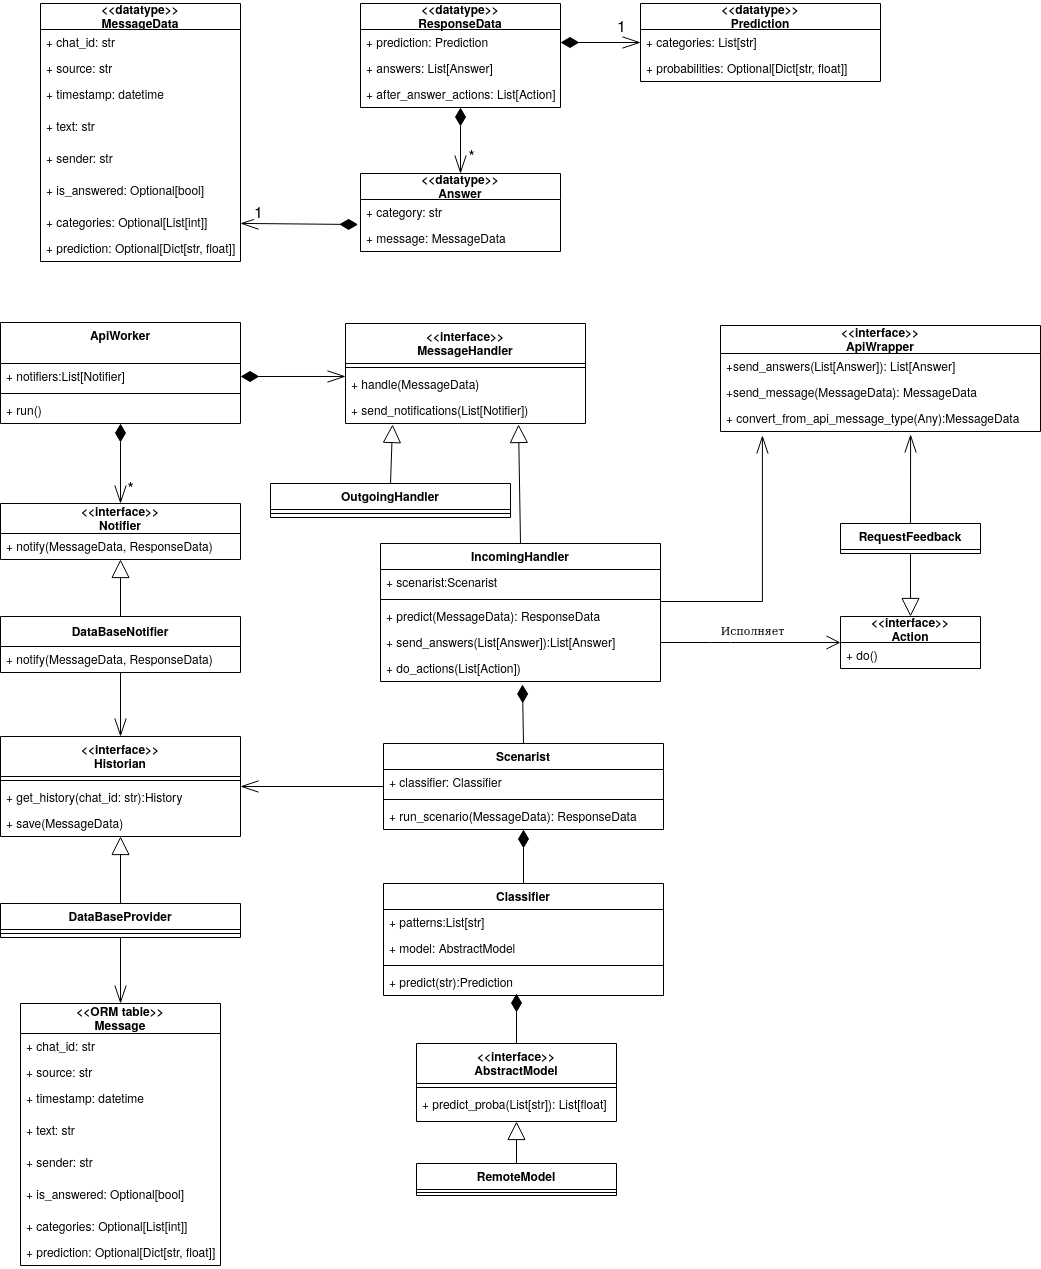
\includegraphics[width=\linewidth]{static/ClassDiagram.png}
        \caption{Диаграмма классов проекта}
        \label{fig:class-diagram}
    \end{figure}

    % Диаграмма процесса обработки сообщения представлена на рисунке ниже.
    % \begin{figure}[!h]
    %     \centering
    %     % TODO Диаграмма процесса
    %     % \includegraphics[width=\linewidth]{}
    %     \caption{Диаграмма процесса обработки сообщения}
    %     \label{fig:func-schema-before}
    % \end{figure}

    \subsection*{Вывод по главе 2}
    В этой главе мы сформулировали основную концепцию нашей будущей системы, 
    описали основные её сущности и способы их взаимодействия. Мы в коде описали 
    сигнатуры их публичных методов базовых классов.
    % , и изобразили основные классы и процессы на диаграммах.
    Теперь, мы можем приступать к их реализации в каждом конкретном канале.

    % реализация
    \section{РЕАЛИЗАЦИЯ}
    \subsection{Уведомления}
    Выполнение несрочных задач в проекте выполняется менеджером отложенных задач \textit(Celery):
    это широко известный кроссплатформенный проект с открытым исходным кодом на Python для
    асинхронного выполнения задач через вызов удаленных процедур.
    В качестве брокера задач мы используем RabbitMQ\cite{docs.rabbitmq}.
    Для добавления задач в очередь в нашем проекте используются "уведомления" (\inlinecode{Notifier}).
    Перечислим все виды уведомлений, которые существуют на настоящий момент:
    \begin{itemize}
        \item \inlinecode{DataBaseMessageNotifier} -- сохранение сообщения в базу;
        \item \inlinecode{DataBaseResponseNotifier} -- сохранение ответов в базу;
        \item \inlinecode{DataBaseCarefulNotifier} -- сохранение сообщения в базу, если оно ещё не существует;
        \item \inlinecode{AppLogerNotifier} -- уведомление о некоторых событиях в мессенджер.
    \end{itemize}
    Пример реализации сохранения в базу представлен на листинге ниже.

    \begin{figure}[!h]
        \centering
        \lstinputlisting[language=Python]{snippets/data_base_message_notifier.py}
        \caption{Код класса DataBaseMessageNotifier}
        \label{fig:data_base_message_notifier}
    \end{figure}

    Сама Celery-задача выглядит следующим образом:

    \begin{figure}[!h]
        \centering
        \lstinputlisting[language=Python]{snippets/celery_task.py}
        \caption{Код метода-задачи Celery save_to_db}
        \label{fig:celery_task}
    \end{figure}

    \subsection{Работа с базой}
    В работе с базой данных участвуют две сущности: объектно-реляционная модель Message
    и класс инкапсулирующий работу с базой DBProvider.

    \newpage
    Модель Message выглядит следующим образом:

    \begin{figure}[!h]
        \centering
        \lstinputlisting[language=Python]{snippets/message_model.py}
        \caption{Код ОРМ класса Message}
        \label{fig:message_model}
    \end{figure}

    DBProvider -- это довольно большой статический класс, реализующий как получение истории сообщений,
    так и сохранение новых сообщений в базу.
    Структура класса приведена на листинге ниже.

    \begin{figure}[!h]
        \centering
        \lstinputlisting[language=Python]{snippets/dbprovider.py}
        \caption{Код класса DBProvider}
        \label{fig:dbprovider}
    \end{figure}

    Рассмотрим подробнее методы этого класса:
    \begin{itemize}
        \item \inlinecode{get_history} -- публичный метод для получения истории диалога, осуществляет
        безопасную выгрузку истории чата из базы данных, обрабатывая возникающие исключения;
        \item \inlinecode{_load_history} -- приватный метод, реализующий непосредственную загрузку истории из базы,
        устанавливает временной диапазон истории и формирует результат в надлежащий вид;
        \item \inlinecode{get_latest_datetime} -- метод получения информации о времени последнего сообщения
        в канале или чате, от пользователя, оператора или бота;
        \item \inlinecode{save} -- сохранение нового сообщения в базе, реализует SQL-функцию \inlinecode{INSERT};
        \item \inlinecode{get_or_create} -- создание записи о сообщении в базе, если в этом канале сообщения с таким
        идентификатором ещё не существует, реализует SQL-функцию \inlinecode{IF NOT EXISTS INSERT};
        \item \inlinecode{update_or_create} -- обновление записи в базе о сообщении определенного канала с таким
        идентификатором, либо создание новой записи, реализует SQL-функцию \inlinecode{IF EXISTS UPDATE ELSE INSERT};
        \item \inlinecode{_save} -- непосредственная реализация трех перечисленных выше функций,
        выбирая нужный метод библиотеки \textit{Django} подставляет нужные фильтры поиска и значения для создания
        или обновления записи.
    \end{itemize}

    \subsection{Датаклассы}
    С версией \textit{Python 3.8} в синтаксис языка были введены так называемые
    датаклассы (\textit{dataclasses}).
    Это усовершенствованный синтаксис для описания собственных типов и структур данных.
    В проекте существуют несколько представителей датаклассов. Опишем отдельно каждого из них.
    \begin{enumerate}
        \item \inlinecode{MessageData} -- датакласс для описания сообщений входящих и исходящих,
        содержит всю необходимую для работы обработчика, сценариста и других классов информацию:
        идентификатор чата, название канала-источника, время получения, отправителя,
        список классифицированных категорий, а также некоторые флаги и идентификаторы.

        \begin{figure}[!h]
            \centering
            \lstinputlisting[language=Python]{snippets/messagedata.py}
            \caption{Код класса MessageData}
            \label{fig:messagedata}
        \end{figure}

        \item \inlinecode{Answer} -- контейнер с ответом бота на входящее сообщение.

        \begin{figure}[!h]
            \centering
            \lstinputlisting[language=Python]{snippets/answer.py}
            \caption{Код класса Answer}
            \label{fig:answer}
        \end{figure}

        \item \inlinecode{Prediction} -- контейнер с результатами классификации текста сообщения,
        которые возвращает классификатор.

        \begin{figure}[!h]
            \centering
            \lstinputlisting[language=Python]{snippets/prediction.py}
            \caption{Код класса Prediction}
            \label{fig:prediction}
        \end{figure}

        \item \inlinecode{ResponseData} -- датакласс со всем, что нужно боту, чтобы корректно
        среагировать на входящее сообщение пользователя.

        \begin{figure}[!h]
            \centering
            \lstinputlisting[language=Python]{snippets/responsedata.py}
            \caption{Код класса ResponseData}
            \label{fig:responsedata}
        \end{figure}

    \end{enumerate}

    \subsection{Канал telegram}
    Так как за обработку отложенных действий теперь отвечает менеджер задач \textit{Celery},
    исчезла потребность в асинхронной обработке сообщений, мы отказались от асинхронности.
    Это позволяет использовать синхронные библиотеки, выбор которых гораздо больше,
    а логика синхронных приложений гораздо проще для понимания.
    В новой реализации telegram-канала была использована другая библиотека -- \textit{pyrogram}\cite{docs.pyrogram}.
    Структура \inlinecode{TelegramWorker} осталась примерно той же: два фильтра событий и две функции, описывающие
    обработку входящих и исходящих сообщений подаются в цикл обработки событий (\textit{event loop})
    telegram клиента.
    Обработка сообщений заключается в их преобразовании во внутренний тип \inlinecode{MessageData}
    и передаче обработчику в \inlinecode{IncomingHandler} или в \inlinecode{OutgoingHandler}.
    \inlinecode{TelegramApiWrapper} наследуется от базового класса \inlinecode{ApiWrapper},
    реализует его абстрактные методы \inlinecode{send_message} и \inlinecode{convert_from_api_message_type}.

    \subsection{Канал ВКонтакте}
    Для реализации канала ВКонтакте используется
    библиотека \textit{vk\_api}\cite{docs.vkapi}.
    Для получения сообщений используется технология LongPoll, в которой, после
    установления соединения и начала сессии, клиент получает
    от сервера ВКонтакте уведомления о всех новых событиях в беседе.
    У каждого нового события проверяется
    является ли оно сообщением, а также поле \inlinecode{to_me}, из которого определяется каким образом
    должно обрабатываться сообщение, как входящее или исходящее.
    Обработка сообщений, также как и в случае с telegram, заключается в их преобразовании во внутренний тип
    и передаче одному из обработчиков.

    \subsection{Канал почты}
    Ввиду отсутствия у библиотек по работе с почтой инструментов, похожих на LongPoll, этот инструмент был
    создан самостоятельно. Для этого мы поочередно просматриваем папки входящей и исходящей почты на наличие
    непрочитанных и необработанных ботом сообщений. Также был объявлен специальный датакласс \inlinecode{EmailMessage}
    канала почты, со специальными полями, и класс \inlinecode{EmailMessageBuilder} для создания объекта датакласса.
    Дополнительно были созданы классы обертки над библиотеками \textit{imap} и \textit{smtp}, в которых
    реализован алгоритм установления и проверки соединения и переподключения в случае его разрыва.
    На почте присутствует сложная логика, связанная пометкой обработанных ботом сообщений флажком
    и перекладыванием отвеченных сообщений в отдельную папку. Дополнительно ситуация осложняется тем, что
    одновременно в одном почтовом ящике могут работать кроме бота ещё два оператора и сторонний парсер почты,
    из-за чего часто возникают конфликтные ситуации. Ситуации могут выражаться, например в прочтении и снятии флага
    \inlinecode{unseen} с писем, предназначенных для бота, и так далее. Поэтому обработка писем в этом канале перегружена
    различными дополнительными проверками.

    \subsection{Сценарист и сценарии}
    Диалоговая система в целом не перенесла существенных изменений, так как целью рефакторинга не ставилось
    улучшение точности или полноты распознавания. Изменения претерпел только модуль для сборки модели.
    Он был перенесен в рабочий проект целиком, практически без изменений, в корневую директорию нового проекта.
    В первую очередь, это было нужно, чтобы решить проблему импортов библиотек при распаковке модели.
    Дело в том, что для сериализации модели в проекте используется библиотека \textit{joblib}, которая при сериализации
    классов, использованных в составе модели, сохраняет путь импортов, а при десериализации использует эти же пути
    для восстановления модели в оперативной памяти.
    Проблема заключается в том, что пути импортов сохраняются относительно точки запуска скрипта сборки, или,
    в нашем случае, \textit{jupyter} тетрадки с кодом сборки. Соответственно, если точка входа в приложение
    будет находится в другом каталоге, импорты провалятся и приложение завершится с ошибкой.
    Размещение скриптов для сборки модели и запуска приложения в одном каталоге -- самое легкое и очевидное
    решение, в дальнейшем позволяет не отвлекаться на проблему загрузки модели во время работы над ней.

    \subsection{Обработчик}
    Для обработки сообщений был реализован базовый класс \inlinecode{MessageHandler}, в котором объявлен
    абстрактный метод \inlinecode{handle()} и реализован общий для входящих и исходящих сообщений
    метод \inlinecode{notify}, который рассылает уведомления всем заявленным уведомителям.
    Метод \inlinecode{handle()} содержит реализуется в виде перечня последовательных действий,
    которые должны быть проделаны над сообщением.

    В \inlinecode{IncomingHandler} это вызов сценариста для формирования ответа, отправка ответных сообщений,
    отправка уведомлений, выполнение дополнительных действий. Листинг метода представлен ниже.

    \begin{figure}[!h]
        \centering
        \lstinputlisting[language=Python]{snippets/incomig_handler_handle.py}
        \caption{Код класса IncomingHandler}
        \label{fig:incomig_handler_handle}
    \end{figure}

    В \inlinecode{OutgoingHandler} никаких действий кроме отправки уведомлений не требуется.
    Реализация этого класса представлена ниже.

    \begin{figure}[!h]
        \centering
        \lstinputlisting[language=Python]{snippets/outgoing_handler.py}
        \caption{Код класса OutgoingHandler}
        \label{fig:outgoing_handler}
    \end{figure}

    \subsection*{Вывод по главе 3}
    В этой главе мы описали все реализованные нами классы и методы, объяснили принципы
    их работы и перечислили некоторые связанные с ними нюансы.
    Для наглядности мы привели листинги кода.
    В ходе самой разработки были решены основные проблемы, перечисленные в первой главе данной работы.
    Проект переписан с единой архитектурой для всех каналов чат-бота что улучшает понимание и поддержку
    проекта, для работы с базой теперь используется объектно-реляционная модель, что также сильно
    упрощает поддержку и написание нового функционала,
    проект полностью снабжен аннотациями типов, что позволяет проводить статический анализ.

    % тестирование
    \section{ТЕСТИРОВАНИЕ}
    \subsection{Статический анализ}
    Для статического анализа соответствия типов в Python используются аннотации 
    из встроенного модуля \inlinecode{typing} и специальный линтер и анализатор.
    Существует несколько анализаторов,
    и \textit{mypy} \cite{docs.mypy} - наиболее популярный из них.
    Он полностью написан на Python, поддерживается и развивается открытым
    сообществом 
    и Гвидо ван Россумом (\textit{Guido van Rossum} \cite{guido.van.rossum})
    в частности. Поэтому проект быстрее получает поддержку новых изменений в
    синтаксисе языка, что особенно важно для нас, так как в проекте на данный
    момент используются последняя мажорная версия Python 3.8.

    Так как многие Python сторонние библиотеки уже написаны без использования
    аннотации типов, их дополняют заголовочными модулями,
    так называемыми \textit{stub}-файлами. В таком случае, статическую типизацию
    можно использовать даже с изначально динамически типизированными модулями.
    
    \textit{Mypy} может использоваться как консольная утилита,
    как линтер, подсказывая ошибки и предложения использования переменных и 
    функций в IDE, 
    но также может генерировать полноценные отчеты, как на примере ниже.
    \begin{figure}[H]
        \centering
        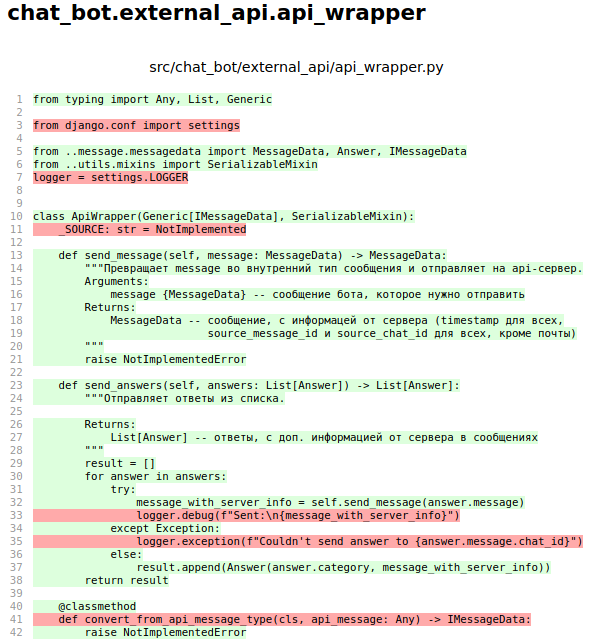
\includegraphics[width=\linewidth]{static/mypy-report.png}
        \caption{Отчет \textit{mypy} в формате html}
        \label{fig:mypy-report}
    \end{figure}
    
    \subsection{Автоматические тесты}
    Во время работы над проектом активно использовались модульные,
    интеграционные и системные тесты. \cite{test.kulikov}
    Для написания модульных тестов использовалась
    встроенная библиотека \textit{unittest} \cite{test.unittest}.
    Обязательными модульными тестами покрываются все публичные методы классов,
    приватные методы тестируются по мере их необходимости.
    Для интеграционных тестов,
    там где было необходимо проверить взаимодействие приложения с базой данных,
    использовалась библиотека \textit{django.test} фреймворка \textit{django}
    \cite{docs.django}.
    Для системных тестов, а именно проверки корректности работы веб-API
    приложения, использовалась библиотека \textit{tavern} \cite{test.tavern}.
    Сами тесты \textit{tavern} описываются в документе в формате yaml, при этом
    могут быть описаны адрес и содержимое запроса и
    проверены как код ответа сервера и его содержимое.
    Пример описания документа с тестом приведен на листинге ниже.
    \begin{figure}[H]
        \centering
        \lstinputlisting{snippets/tavern-test.yaml}
        \caption{Конфигурационный файл Tavern тестов}
        \label{fig:tavern-tests}
    \end{figure}

    Все тесты полностью автоматизированы, для этого использовался
    фреймворк \textit{pytest} \cite{test.pytest},
    предоставляющий библиотеку для написания тестов и
    утилиту для их запуска. Но в первую очередь фреймворк был выбран из-за его
    возможности объединять и совместно выполнять тесты
    \textit{unittest}, \textit{django.test} и \textit{tavern}.
    Всего в проекте зарегистрировано 209 модульных и интеграционных тестов и
    5 системных.

    \subsection{Нагрузочное тестирование}
    Нагрузочное тестирование проводилось на тестовом сервере на полностью
    развернутом веб-приложении с веб-сервером \textit{Nginx} при помощи
    инструмента Яндекс.Танк \cite{test.yandex.tank}.
    Целью нагрузочного тестирования было установление
    порога стабильной работы сервиса. Для этого на него подавалась нагрузка
    с константным количеством запросов в секунду в течение 2 минут с итеративным
    увеличением количества запросов.

    Конфигурационный файл для Яндекс.Танка:
    \begin{figure}[H]
        \centering
        \lstinputlisting{snippets/load.yaml}
        \caption{Конфигурационный файл Яндекс.Танка}
        \label{fig:tank-load}
    \end{figure}

    Так, было установлено, что сервис стабильно выдерживает нагрузку до 18
    запросов в секунду в течение 2 минут.
    % TODO какой-нибудь график

    \subsection*{Вывод по главе 4}
    В этой главе мы рассмотрели виды тестирования, реализованные в новом проекте.
    В проекте были использованы модульные, интеграционные, системные и нагрузочные
    тесты для исследования и контроля за соответствием продуктом требуемых
    поведения и производительности,
    что в дальнейшем поможет в развитии и поддержке проекта.

    % развертывание и внедрение
    % \section{РАЗВЕРТЫВАНИЕ И ВНЕДРЕНИЕ}

    % сравнительный анализ сложности проектов
    \section{АНАЛИЗ ПРОЕКТОВ}
    \subsection{Метрики}

    \subsection{Сравнение}
    
    \begin{table}[!h]
        \caption{Сравнение метрик программного обеспечения проектов}
        \begin{center}
            \begin{tabular}{l|r|r}
                \textbf{Метрика} & \textbf{Исходный} & \textbf{Конечный} \\
                \hline
                Количество строк кода               & 7436 & 5886 \\
                Количество модулей                  & 67 & 87 \\
                Среднее число строк на модуль       & 110.985 & 67.655 \\
                Количество классов и интерфейсов    & 100 & 182 \\
                Цикломатическая сложность           & & \\
                Анализ функциональных точек         & & \\
                Степень покрытия кода тестированием & & \\
                Покрытие требований                 & & \\
                Метрики программного пакета от      & & \\
                Роберта Сесиль Мартина              & & \\
                Связность                           & & \\
            \end{tabular}
        \end{center}
    \end{table}

    \subsection{Выводы}

    % заключение
    \addcontentsline{toc}{section}{ЗАКЛЮЧЕНИЕ}
\section*{ЗАКЛЮЧЕНИЕ}
Целью данной работы было проведение работ по улучшению
функциональности, надежности, читаемости и модифицируемости существующего проекта
чат-бота. Для достижения этой цели был проведен анализ исходного проекта, выявление
его недостатков, составление плана работ с перечнем требуемых характеристик конечного
результата.

По итогу выполнения работ была получен единый цельный проект, с четко прописанной архитектурой,
использующий удобные и понятные средства по работе с базой данных и
системой отложенного выполнения задач.
Поскольку работы велись по принципу разработки через тестирование, проект максимально покрыт
функциональными и unit-тестами.

    % литература
    \addcontentsline{toc}{section}{Библиографический список}
    \printbibliography[title={Библиографический список}]

\end{document}